%==============================================================================
% Sjabloon poster bachproef
%==============================================================================
% Gebaseerd op document class `a0poster' door Gerlinde Kettl en Matthias Weiser
% Aangepast voor gebruik aan HOGENT door Jens Buysse en Bert Van Vreckem

\documentclass[a0,portrait]{hogent-poster}

% Info over de opleiding
\course{Bachelorproef}
\studyprogramme{toegepaste informatica}
\academicyear{2025-2026}
\institution{Hogeschool Gent, Valentin Vaerwyckweg 1, 9000 Gent}

% Info over de bachelorproef
\title{Optimalisatie van het beheer van leeggoedpalletten bij Freshfrozen For Pets}
\subtitle{Een onderzoek naar een digitale oplossing voor foutenreductie en gebruiksvriendelijkheid}
\author{Wout Schelstraete}
\email{wout.schelstraete@student.hogent.be}
\supervisor{Mevr. L. Lewyllie}
\cosupervisor{Dhr. P. Kemseke (Freshfrozen For Pets)}

% Indien ingevuld, wordt deze informatie toegevoegd aan het einde van de
% abstract. Zet in commentaar als je dit niet wilt.
%\specialisation{Systeem- en Netwerkbeheer}
%\keywords{Leeggoedbeheer, ERP, Blazor WebAssembly, KMO, Foutenreductie}
%\projectrepo{https://github.com/user/repo}

\begin{document}

\maketitle

\begin{abstract}
Freshfrozen For Pets is een West-Vlaamse KMO die verse maaltijden voor honden en katten produceert. Leveringen komen binnen op of in leeggoed dat na gebruik teruggestuurd moet worden naar de leverancier. Dat leeggoed wordt vandaag volledig in Microsoft Excel beheerd, met per leverancier een eigen spreadsheet. Die werkwijze is foutgevoelig: invoer is niet afdwingbaar, waarden worden destructief overschreven, er is geen historiek en het ERP-systeem kent het leeggoed niet. Deze bachelorproef onderzoekt hoe dat beheer efficiënter kan, met focus op tijdsbesparing, foutenreductie, gebruiksvriendelijkheid en overzichtelijkheid. Drie scenario's werden uitgewerkt: een directe integratie in het bestaande ERP, een middleware-koppeling en een standalone-applicatie (proof-of-concept met Blazor WebAssembly, ASP.NET en PostgreSQL). De optimale oplossing combineert de overzichtelijke modules van de eigen applicatie met de afdwingbaarheid van een directe integratie in het ERP-systeem.
\end{abstract}

\begin{multicols}{2} % This is how many columns your poster will be broken into, a portrait poster is generally split into 2 columns

\section{Introductie}

Freshfrozen For Pets is een KMO die verse maaltijden voor huisdieren produceert. Voor die productie wordt vlees geleverd door meerdere leveranciers. De bestellingen komen binnen op \emph{leeggoed} (pallets) dat na gebruik terug naar de leverancier moet. Wie welk leeggoed nog tegoed heeft, wordt bijgehouden in Excel, met per leverancier een apart bestand.
\\
Het beheer in Excel brengt structurele risico's met zich mee:
\begin{itemize}
    \item De invoer is op geen enkel moment \textbf{afdwingbaar}, waardoor leeggoedbewegingen vergeten worden.
    \item Waarden worden \textbf{destructief overschreven}: er is geen historiek of audit-spoor.
    \item De data is \textbf{versnipperd} over losse spreadsheets, een totaaloverzicht ontbreekt.
\end{itemize}
Onopgemerkte fouten leiden tot administratieve inefficiëntie en financieel verlies via een incorrecte teruggave van statiegeld.

\section{Onderzoeksvraag}

``Hoe kan het beheer van leeggoed bij Freshfrozen For Pets efficiënter georganiseerd worden, met als focus om tijdbesparing, foutenreductie, procesmatige gebruiksvriendelijkheid en overzichtelijkheid te verbeteren?''

\section{Methodologie}

Het onderzoek start met een \textbf{intern onderzoek} (fase 0) bij Freshfrozen: interviews met de CEO, de productiechef en een financieel bediende, een enquête bij de dagelijkse gebruikers en overleg met ERP-leverancier MAPA. Daarna worden drie technologische scenario's onderzocht:

\begin{enumerate}
    \item \textbf{Directe integratie}. Leeggoedbeheer rechtstreeks in het bestaande ERP-systeem.
    \item \textbf{Middleware}. Een apart leeggoedsysteem dat via een point-to-point-integratie met het ERP communiceert.
    \item \textbf{Standalone-applicatie}. Een onafhankelijke proof-of-concept (PoC).
\end{enumerate}

Uit het overleg met MAPA bleek dat een concrete uitvoering van fase 1 en fase 2 niet mogelijk was door licentie- en codebase-restricties. Deze fases werden daarom theoretisch uitgewerkt. De PoC van fase 3 werd wel volledig geïmplementeerd en iteratief gevalideerd met een eindgebruiker.

\section{De proof-of-concept (Fase 3)}

De PoC is gebouwd met een Blazor WebAssembly-frontend bovenop een ASP.NET-API met een PostgreSQL-database. De applicatie biedt onder meer:

\begin{itemize}
    \item Een \textbf{stockoverzicht} dat per leverancier en leeggoedtype het openstaande tegoed toont.
    \item Een \textbf{stockhistoriek} met datumbereik, bronfilter en kleurgecodeerde bewegingen, zodat foute bewegingen teruggevonden worden.
    \item Validatie aan \textbf{client- en serverzijde}, wederzijds filterende dropdowns en een bevestigingsstap bij verdacht grote correcties.
\end{itemize}

\begin{center}
  \captionsetup{type=figure}
  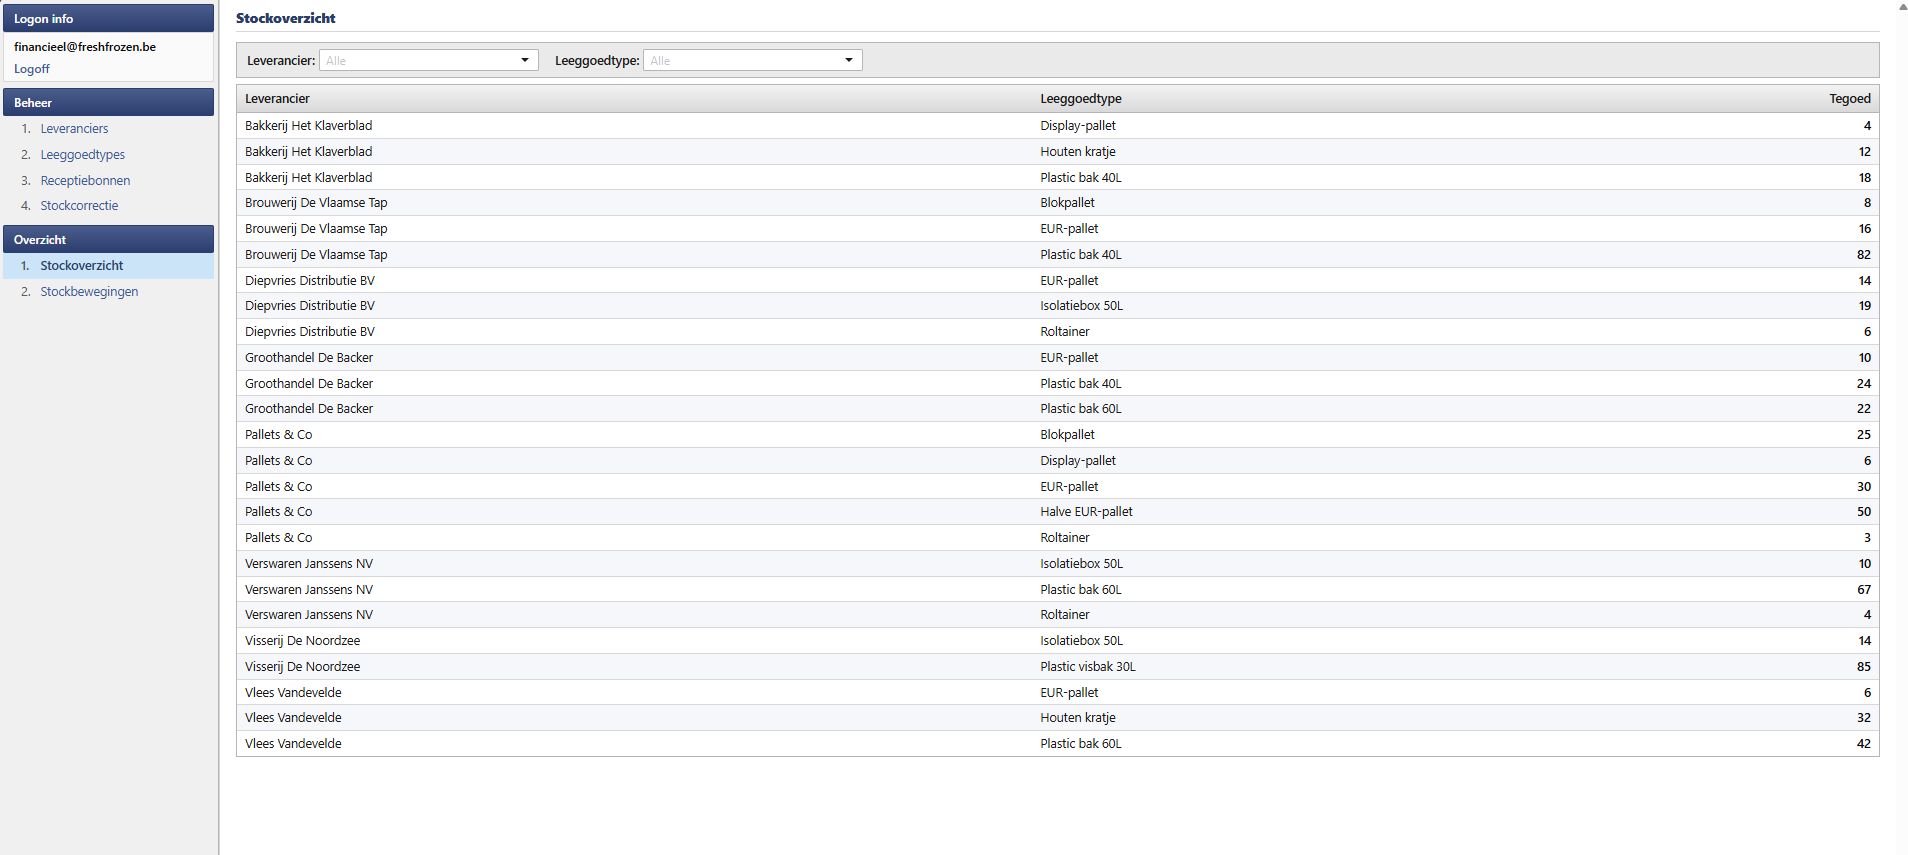
\includegraphics[width=1.0\linewidth]{../bachproef/images/poc/stockoverzicht}
  \captionof{figure}{Stockoverzicht van de PoC: het openstaande tegoed per leverancier en per leeggoedtype, met wederzijds filterende dropdowns.}
\end{center}

\section{Resultaten}

De PoC werd geëvalueerd op de vier pijlers van de onderzoeksvraag:

\begin{itemize}
    \item \textbf{Overzichtelijkheid:} alle data op één plek, opgedeeld in eigen modules.
    \item \textbf{Gebruiksvriendelijkheid:} verkozen boven Excel, dankzij vertrouwde ERP-terminologie en User-Centric Design.
    \item \textbf{Foutenreductie:} validatie, logging en historiek zijn een goede toevoeging, maar de manuele ingave voor referentiecodes van receptiebonnen en geen mogelijkheid tot afdwingen van invoer blijft een knelpunt.
    \item \textbf{Tijdsbesparing:} winst bij het raadplegen, maar verlies door de manuele ingave van referentiecodes van receptiebonnen.
\end{itemize}

De zwakke punten van de standalone-applicatie (geen afdwingbaarheid, een tweede systeem naast het ERP, dubbele invoer) zijn net de sterktes van een directe integratie in het ERP.

\section{Conclusie}

Het beheer van leeggoed kan het efficiëntst georganiseerd worden door de modules en gebruikerservaring van de eigen applicatie (fase 3) verder te laten uitwerken binnen het bestaande ERP-systeem van MAPA (fase 1)}. Zo worden de afdwingbaarheid en het ontbreken van datasilo's uit fase 1 gecombineerd met de overzichtelijkheid en gebruiksvriendelijkheid uit fase 3, en worden de vier pijlers van de onderzoeksvraag tegelijk beantwoord.

\section{Toekomstig onderzoek}

De uitwerking van fase 1 en de screenshots van de PoC worden met MAPA gedeeld als concreet vervolgtraject voor Freshfrozen. Elke case is echter anders: deze drie implementatiemethodes vormen een leidraad, geen definitief antwoord op elk bedrijfsproces. Een proces dat los staat van een bestaand systeem kan beter wel standalone uitgewerkt worden.

\end{multicols}
\end{document}
